\documentclass[tikz]{standalone}
\renewcommand*\familydefault{\sfdefault}
\usetikzlibrary{calc,trees,positioning,arrows,chains,shapes.geometric,%
    decorations.pathreplacing,decorations.pathmorphing,shapes,%
    matrix,shapes.symbols,fit}

\pgfdeclarelayer{back}
\pgfsetlayers{back,main}


\makeatletter
\tikzset{
  fitting node/.style={
    inner sep=0pt,
    fill=none,
    draw=none,
    reset transform,
    fit={(\pgf@pathminx,\pgf@pathminy) (\pgf@pathmaxx,\pgf@pathmaxy)}
  },
  reset transform/.code={\pgftransformreset},
  node/.append style={text color=white, color=white}
}
\makeatother


\begin{document}
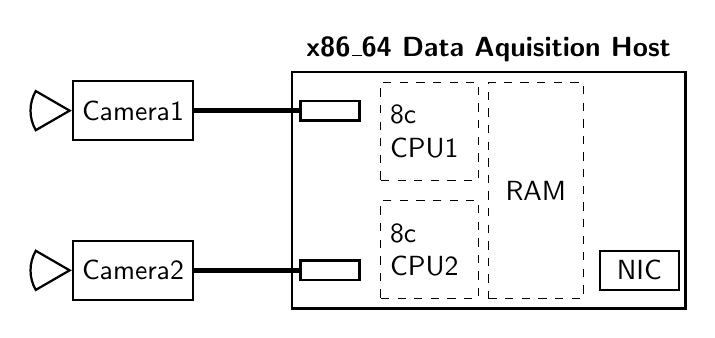
\begin{tikzpicture}[%every node/.style={color=white}
]

  \node [draw,thick,rectangle, minimum width=5cm, minimum height=3cm] at(0,0) (host) {};
  \node [anchor=south] at($(host.north)$) {\bfseries{}x86\_64 Data Aquisition Host};

  \node [draw,thick,rectangle, minimum width=1cm, minimum height=.75cm] at($(host.north west) - (2,.5)$) (cmos1) {Camera1};
  \node [draw,thick,rectangle, minimum width=1cm, minimum height=.75cm] at($(host.south west) - (2,-.5)$) (cmos2) {Camera2};

  \node [draw,thick,rectangle, minimum width=.75cm, minimum height=.25cm] at($(host.north west) + (.5,-.5)$) (fg1) {};
  \node [draw,thick,rectangle, minimum width=.75cm, minimum height=.25cm] at($(host.south west) + (.5,.5)$) (fg2) {};

  \draw [ultra thick] (cmos1) -- (fg1);
  \draw [ultra thick] (cmos2) -- (fg2);

  \node [circular sector,  thick, shape border uses incircle, draw,anchor=east] at($(cmos1.west)$) (lens1) {};
  \node [circular sector,  thick, shape border uses incircle, draw,anchor=east] at($(cmos2.west)$) (lens2) {};

  \node [draw,dashed,rectangle, minimum width=1.2cm, minimum height=1.25cm, text width=1cm] at($(host) - (.75,0) + (0,.75)$) (cpu1) {8c CPU1};
  \node [draw,dashed,rectangle, minimum width=1.2cm, minimum height=1.25cm, text width=1cm] at($(host) - (.75,0) - (0,.75)$) (cpu2) {8c CPU2};

  \node [draw,dashed,rectangle, minimum width=1.2cm, minimum height=2.75cm] at($(host) + (.6,0)$) (ram) {RAM};

  \node [draw,thick,rectangle, minimum width=1cm, minimum height=.5cm] at($(host.south east) + (-.6,.5)$) (nic) {NIC};
  
\end{tikzpicture}
\end{document}
